% *******************************************************************************
% * Copyright (c) 2007 by Elexis
% * All rights reserved. This document and the accompanying materials
% * are made available under the terms of the Eclipse Public License v1.0
% * which accompanies this distribution, and is available at
% * http://www.eclipse.org/legal/epl-v10.html
% *
% * Contributors:
% *    G. Weirich - initial implementation
% *
% *  $Id: konsviews.tex 4902 2009-01-03 10:47:34Z rgw_ch $
% *******************************************************************************
% !Mode:: "TeX:UTF-8" (encoding info for WinEdt)


\section{Konsultationsbezogene Views}



\subsection{Fälle}
Diese View (Abb. \ref{fig:faelle2} listet alle für den aktuell selektierten
Patienten existierenden Fälle. \index{Fall-Liste}
\begin{wrapfigure}{l}{6.8cm}
  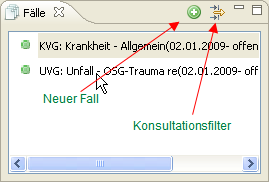
\includegraphics{images/faelleview}
  \caption{Fälle - View}
  \label{fig:faelle2}
\end{wrapfigure}

Das Symbol links von der Fallbezeichnung gibt an, ob alle für die Verrechnung
des Falles notwendigen Daten vorhanden sind: Wenn es grün ist, sollte die
Rechnungserstellung möglich sein, wenn es rot ist, fehlen noch eine oder mehrere
Angaben.

\textit{Welche} Angaben mindestens notwendig sind, hängt vom Abrechnungssystem ab. So ist für Fälle, die nach dem KVG abgerechnet werden, die Angabe
eines Rechnungsempfängers, eines Versicherers und der Versichertennummer
notwendig. Bei Fällen, die nach UVG abgerechnet werden, muss eine Fallnummer
vorhanden sein. Bei Privatrechnungen wird mindestens ein Rechnungsempfänger anzugeben sein.

\medskip

\index{konsultationen!filtern}
\label{filter:fall}
Klick auf das Filtersymbol in der Titelzeile der View führt dazu, dass nu noch diejenigen Konsultationen in der Konsultationsliste (siehe \ref{view:konsultationen}) angezeigt werden, welche zum gerade ausgewählten Fall gehören. Wenn ein anderer Fall angeklickt wird, wird die Liste erneut gefiltert. Erneuter Klick auf das Filter-Symbol schaltet den Filter wieder aus.

Rechtsklick auf einen Fall öffnet dessen Kontextmenü. Dieses enthält die
folgenden Punkte:
\begin{itemize}
  \item {Fall löschen}. Dies ist nur möglich, wenn Sie die dazu notwendigen Rechte
  haben, und wenn zu diesem Fall keine Konsultationen mehr existieren.
  \item {Fall bearbeiten}. Dies öffnet eine weitere View, in der Details zum
  aktuell ausgewählten Fall eingegeben werden können.
  \item {Fall wieder öffnen}. Damit kann man einen bereits
  geschlossenen\footnote{Ein Fall ist dann geschlossen, wenn ein End-Datum
  eingegeben wurde. Zu einem geschlossenen Fall können keine Konsultationen mehr
  hinzugefügt werden.} Fall wieder öffnen.
  \item {Rechnung erstellen}. Hiermit lässt sich über alle unverrechneten
  Konsultationen des aktuellen Falls und des aktuellen Mandanten eine Rechnung
  erstellen. Dies ist eine \glqq Abkürzung\grqq{} des normalen Wegs der
  Rechnungserstellung und eignet sich vor allem für Sofortrechnungen einzelner
  Konsultationen oder Leistungen.
\end{itemize}


\clubpenalty=5000

\subsection{Fälle und Kons}
 %\usepackage{graphics} is needed for \includegraphics
\begin{wrapfigure}{l}{7cm}
  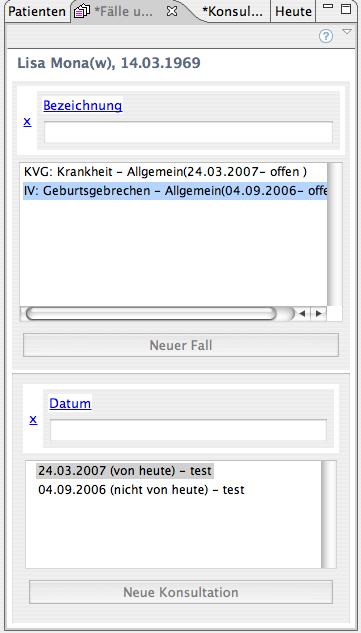
\includegraphics[width=7cm]{images/fallkonsview}
  \caption{Fälle und Kons}
  \label{fig:fallkons}
\end{wrapfigure}
Diese View (Abb. \ref{fig:fallkons} listet synoptisch Fälle und dazugehörige
Konsultationen (Nur Titel ohne Texte) auf. Wenn im oberen Bereich ein Fall
angeklickt wird, werden im unteren Bereich die zu diesem Fall gehörenden
Konsultationen angezeigt. Wenn eine Konsultation angeklickt wird, wird diese
Konsultation in der Konsultation-View (S. \ref{konsview} s. \pageref{konsview}) angezeigt.

Um einen neuen Fall zu erstellen, geben Sie einen Titel für diesen Fall ein und klicken dann auf \textit{neuer Fall}. Um eine neue Konsultation einzugeben, wählen Sie den dazugehörigen Fall aus und klicken auf \textit{Neue Konsultation}

\medskip

Anmerkung: Sie werden festgestellt haben, dass diese View und die vorher besprochene Fälle-View bis zu einem gewissen Punkt redundant sind. Das ist auch so. Sie können getrennte Views für Fälle und Konsultationen bevorzugen, oder eine View in der beides enthalten ist. In der Regel werden Sie nicht beide Konzepte anwenden, sondern dasjenige, welches Ihnen besser gefällt - Elexis lässt Ihnen die Wahl.

\clearpage

\subsection{Konsultationen}
\label{view:konsultationen}
\begin{wrapfigure}{L}{7.5cm}
  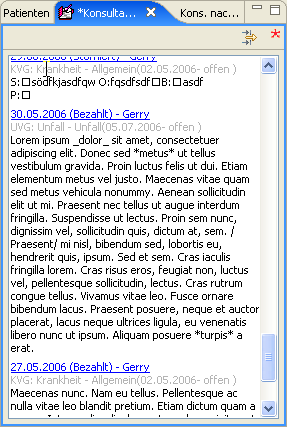
\includegraphics{images/konslisteview}
  \caption{Konsultationsliste}
  \label{fig:konslisteview}
\end{wrapfigure}

Dies ist eine Auflistung aller bisherigen Konsultationen des aktuell
selektierten Patienten, unabhängig vom jeweiligen Fall.
\index{Konsultationsliste} Zu jeder Konsultation
wird der Text ohne Formatierungen angezeigt. (S. Abb. \ref{fig:konslisteview}).\\
Klick auf den (blauen) Titel einer Konsultation wählt diese Konsultation in der
Konsultation-View (s. S. \pageref{konsview}) aus.

Klick auf das Filter-Symbol rechts oben öffnet den Filter-Dialog (s. Abb. \ref{fig:konsfilter}).
\index{Konsultationsfilter} Hier können Sie bestimmte Kriterien eingeben, nach
denen die angezeigten Konsultationen gefiltert werden sollen (d.h. es werden nur
noch diejenigen Konsultationen angezeigt, die den Filterbedingungen
entsprechen).

Im oberen Feld können Sie angeben, ob nur Konsultationen eines bestimmten Falls
oder aller Fälle angezeigt werden sollen. Im unteren Feld können Sie
Suchbegriffe eingeben, welche im Konsultationstext vorkommen müssen. Mehrere
Suchbegriffe können mit AND, OR, NOT, AND NOT und OR NOT miteinander verknüpft werden.
Beispielsweise findet \glqq Lorem AND NOT ipsum\grqq{} nur solche Konsultationen, deren
Text \glqq Lorem\grqq, nicht aber \glqq ipsum\grqq{}enthält.

Ganz unten können Sie schliesslich noch angeben, ob Gross/Kleinschreibung
beachtet werden soll, oder ob Suchbegriffe als reguläre Ausdrücke betrachtet
werden sollen. Eine genaue Erklärung dieses Themas würde hier zu weit führen;
Sie finden sehr viel Literatur dazu mit den Stichwörtern \glqq Regular
Expression\grqq{}oder \glqq Pattern Matching\grqq{}. Diese Technik erlaubt es,
den Suchbegriff mit verschiedensten Platzhaltern zu beschreiben. So würde z.B.
\glqq M[ae][iy]e?r\grqq{} nach allen Meiers, Mayrs etc. in allen Schreibweisen
suchen.

\medskip

Anmerkung:
Das Filtern der Konsultationen mit diesem Verfahren kann, da der Text jeder Konsultstion komplett durchsucht wird, einige Sekunden dauern. Wenn man lediglich nach Fällen oder Problemen filtern möchte, ist der entsprechende Fallfilter (S. \pageref{filter:fall}) oder Problemliste-Filter (S. \pageref{filter:problemliste})im Allgemeinen effizienter.

\begin{figure}[ht]
\begin{center}
  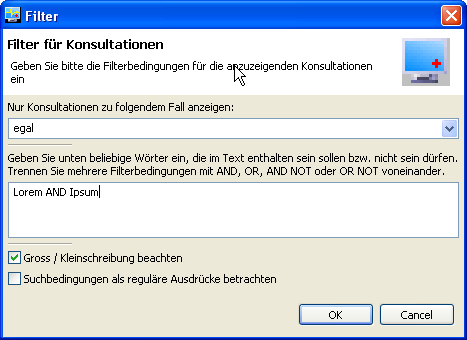
\includegraphics{images/filterdialog}
  \caption{Filterdialog}
  \label{fig:konsfilter}
\end{center}
\end{figure}


\subsection{Konsultation}
 \label{konsview}
Detailansicht eines Konsultationseintrags (S. Abb. \ref{fig:konsdetail}).
\begin{figure}[ht]
  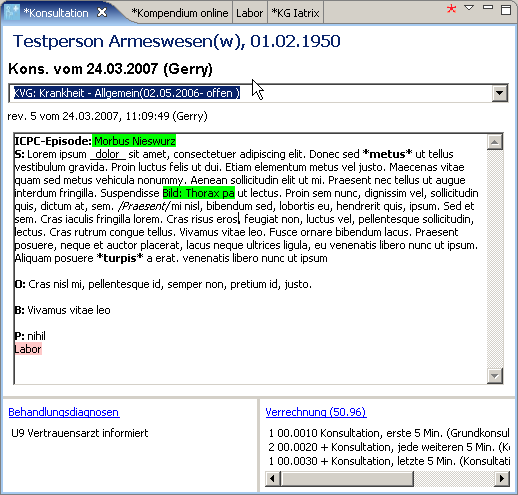
\includegraphics{images/konsview}
  \caption{Konsultation: Detail}
  \label{fig:konsdetail}
\end{figure}

Sie haben im Textfeld folgende zusätzlichen Möglichkeiten:
\begin{description}
\item[Makros]
Schreiben Sie einen beliebigen Text, markieren Sie diesen Text mit der linken Maustaste, klicken Sie dann mit der rechten Maustaste und wählen Sie "'als Makro..."'. eben Sie dem Makro einen beliebigen Namen. Wenn Sie nun zukünftig den Namen des Makros gefolgt von \# tippen, wird dieser Text durch den vorher definierten Inhalt des Makros ersetzt.

\item[Abrechnen]
Wenn Sie den Namen eines Abrechnungsblocks tippen, gefolgt von \#, dann wird dieser Block verrechnet, ebenso, wie wenn Sie ihn mit der Maus ins Verrechnungs-Feld gezogen hätten.

\item[Textauszeichnungen]
Es können auch einige einfache Textauszeichnungen gemacht werden: Ein Wort am Anfang einer Zeile, welches von einem Doppelpunkt gefolgt ist, wird fett gedruckt. Ebenso ein Wort zwischen zwei *. Ein Wort zwischen zwei / wird kursiv geschrieben.
\end{description}


\subsection{AUF}
Diese View dient der Festlegung einer Arbeitsunfähigkeit. (Abb \ref{fig:auf})
\index{AUF} \index{Arbeitsunfähigkeit}.
\begin{figure}
  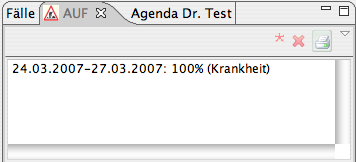
\includegraphics{images/aufview}
  \caption{AUF-View}
  \label{fig:auf}
\end{figure}
Eine AUF bezieht sich immer auf einen bestimmten Fall. Wenn kein Fall markiert
ist, werden Sie aufgefordert, zunächst einen anzugeben.

Wenn Sie auf das \glqq Neu\grqq -Symbol (roter Stern) klicken, erscheint ein
Dialog, in dem Sie Anfang und Ende der neuen Arbeitsunfähigkeit festlegen
können. Klick auf das \glqq Drucker\grqq -Symbol öffnet eine Text-View, in der
Sie noch manuelle Änderungen am AUF-Text ergänzen können, bevor Sie das Zeugnis
definitiv ausdrucken oder aufs Fax senden.

\subsection{Rezepte}
In dieser View werden Rezepte aufgenommen. \index{Rezept}Klicken Sie auf das \glqq Neu\grqq
-Symbol (grünes plus) und es wird ein neues Rezept mit dem Aktuellen Datum
erstellt. Ziehen Sie Artikel mittels Drag\&Drop aus einer Artikelliste oder der
Dauermedikations-View in dieses Rezept. Mit Klick auf das \glqq Drucker\grqq -
Symbol öffnen Sie eine Text-View, in der Sie noch manuelle Änderungen anbringen
können, bevor Sie das Rezept definitiv auf den Drucker oder ein Faxgerät oder in
einen Export-Konnektor senden.
Hierzu muss eine Textvorlage namens \glqq Rezept\grqq
existieren, welche an einer Stelle den Platzhalter [Rezeptzeilen] enthält. Dort
werden die ausgewählten Artikel eingefügt.


\subsection{Falldetail}
\label{falldetail}
\index{Fall!Detailansicht}
Diese View (Abb. \ref{fig:falldetail}) dient zum Einstellen der Details eines Falls (Eine Dialogbox mit derselben View wird geöffnet, wenn man einen neuen Fall (s. \ref{definition:fall} S. \pageref{definition:fall}) erstellt).
\begin{figure}[ht]
  % Requires \usepackage{graphicx}
  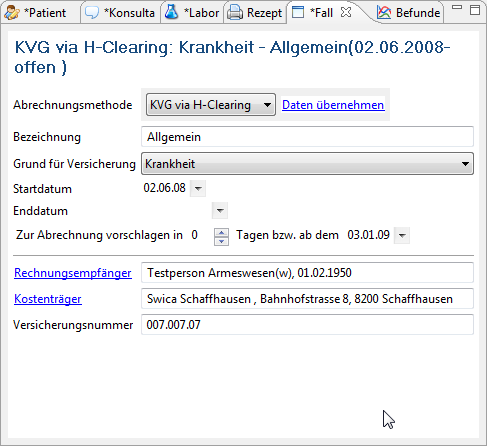
\includegraphics[width=0.8\textwidth]{images/falldetail}\\
  \caption{Fall-Detail}\label{fig:falldetail}
\end{figure}
In der obersten Auswahlbox geben Sie an, welches Abrechnungssystem (S. auch \ref{settings:abrechnungssystem} auf Seite \pageref{settings:abrechnungssystem}) für diesen Fall angewendet werden soll. Darunter steht eine Bezeichnung für den fall, die Sie frei wählen können. Diese dient nur Ihrer eigenen Information, damit Sie verschiedene Fälle desselben Patienten einfacher auseinanderhalten können. Die nächste Zeile, 'Grund für die Versicherung' ist eine Angabe, die auf den zu diesem fall erstellten Rechnungen stehen wird (Falls die Rechnungsvorlage ein entsprechendes Feld enthält).

Das \textbf{Startdatum} ist üblicherweise das Datum der ersten Konsultation, oder bei Unfällen, das Unfalldatum. Das \textbf{Enddatum} hingegen bezeichnet das Datum, wen der Fall abgeschlossen wird. Ein Fall, welcher ein Enddatum hat, wird in der Fall-Liste (Abb. \ref{fig:faelle2}) als 'GESCHLOSSEN' markiert. Zu einem solchen Fall können keine Konsultationen mehr erstellt werden.
In der Regel sollte ein Fall nur abgeschlossen werden, wenn es ein Unfall ist, welcher abgeschlossen ist, oder wenn der Patient den Versicherer wechselt und die Abrechnungsdaten darum ändern.

Die nächste Zeile, Rechnungsempfänger, ist zwingend, damit überhaupt eine Rechnung erstellt werden kann. Dies muss ein bereits existierender Kontakt (z.B. der Patient selbst) sein.

\medskip
Alle weiteren Zeilen sind je nach gewähltem Abrechnungssystem unterschiedlich. Oft wird auch eine Zeile 'Kostenträger' vorhanden sein \footnote{Wichtige Anmerkung für das \textbf{Tarmed-System} (Schweiz): Wenn Rechnungsempfänger und Kostenträger identisch sind, wird eine Tiers Payant-Rechnung erstellt, andernfalls eine Tiers-Garant-Rechnung. Achten Sie also darauf, dass diese beiden Zeilen korrekt sind (Bei UVG-Fällen müssen also sowohl Rechnungsempfänger als auch Kostenträger der jeweilige Unfallversicherer sein, während bei KVG-Fällen in TG-Kantonen der Patient der Rechnungsempfänger und die Krankenkasse der Kostenträger ist)}.

\clearpage

\subsection{Diagnosen}
\label{view:diagnosen} \index{Diagnosen}
Diese View (Abb. \ref{fig:diagnosen}) dient dazu, Diagnosen auszuwählen und einer Konsultation zuzuordnen.
 \begin{wrapfigure}{l}{7cm}
    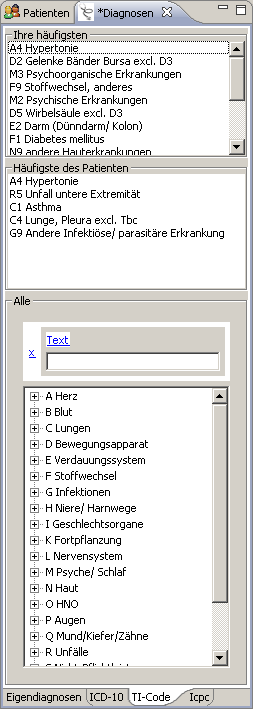
\includegraphics[width=6.5cm]{images/diagnosenview}
    \label{fig:diagnosen}
    \caption{Diagnosen-Auswahl}
\end{wrapfigure}
Unten sehen Sie eine Reihe von Reitern, die den installierten Diagnosecode-Plugins entsprechen (standardmässig TI-Code, ICD-10, und ICPC-2).
Um eine Diagnose auszuwählen, wählen Sie zunächst aus diesen Reitern das entsprechende Codesystem und dann den Code. Die Auswahl kann durch Drag\&Drop oder durch Doppelklick erfolgen.
Für jedes Codesystem sehen Sie ein dreigeteiltes Fenster: Im obersten Bereich sind Ihre (d.h. des aktuell eingeloggten Anwenders) am häufigsten eingesetzten Diagnosen zu sehen; im mittleren Teil diejenigen Diagnosen, die beim aktuell ausgewählten Patienten bisher am häufigsten verwendet worden sind, und um unteren Teil die gesamte Systematik des gewählten Codesystems.

\medskip

Auf diese Weise haben Sie stets Zugriff auf die am häufigsten benötigten Codes und werden nur noch selten die ganze Systematik durchsuchen müssen.

